%%%%%%%%%%%%%%%%%%%%%%%%%%%%%%%%%%%%%%
% TRB Poster 2015
% Created by Subasish Das
% January 2015
%%%%%%%%%%%%%%%%%%%%%%%%%%%%%%%%%%%%%%

\documentclass[final]{beamer}
\usepackage[scale=1.24]{beamerposter}
\usepackage{graphicx}			% allows us to import images

%-----------------------------------------------------------
% Custom commands that I use frequently
%-----------------------------------------------------------

\newcommand{\bb}[1]{\mathbb{#1}}
\newcommand{\cl}[1]{\mathcal{#1}}
\newcommand{\fA}{\mathfrak{A}}
\newcommand{\fB}{\mathfrak{B}}
\newcommand{\Tr}{{\rm Tr}}
\newtheorem{thm}{Theorem}

%-----------------------------------------------------------
% Define the column width and poster size
%-----------------------------------------------------------

\newlength{\sepwid}
\newlength{\onecolwid}
\newlength{\twocolwid}
\setlength{\paperwidth}{48in}
\setlength{\paperheight}{36in}
\setlength{\sepwid}{0.024\paperwidth}
\setlength{\onecolwid}{0.22\paperwidth}
\setlength{\twocolwid}{0.464\paperwidth}
\setlength{\topmargin}{-0.5in}
\usetheme{confposter}
\usepackage{exscale}

%-----------------------------------------------------------
% The next part fixes a problem with figure numbering. Thanks Nishan!
%-----------------------------------------------------------

\usecaptiontemplate{
\small
\structure{\insertcaptionname~\insertcaptionnumber:}
\insertcaption}

%-----------------------------------------------------------
% Define colours (see beamerthemeconfposter.sty to change these colour definitions)
%-----------------------------------------------------------

\setbeamercolor{block title}{fg=Mahogany,bg=white}
\setbeamercolor{block body}{fg=Black,bg=white}
\setbeamercolor{block alerted title}{fg=white,bg=Maroon!70}
\setbeamercolor{block alerted body}{fg=black,bg=Green!10}

%-----------------------------------------------------------
% Name and authors of poster/paper/research
%-----------------------------------------------------------

\title{Zero-inflated Models for Different Severity Types in Rural Two-lane Crashes}
\author{Subasish Das, PhD Candidate \hspace{5in} Xiaoduan Sun, PhD \& PE, Professor}
\institute{University of Louisiana \hspace{10in} University of Louisiana }

%-----------------------------------------------------------
% Start the poster itself
%-----------------------------------------------------------


\begin{document}
\begin{frame}[t]
  \begin{columns}[t]												% the [t] option aligns the column's content at the top
    \begin{column}{\sepwid}\end{column}			% empty spacer column
    \begin{column}{\onecolwid}
      \begin{alertblock}{Research Question}
        {\rmfamily{What are the effects of the key geometric features in crash severity? Are ZINB and ZIP models sufficient to get better prediction?}}
      \end{alertblock}
      \vskip2ex
      \begin{figure}
              \begin{center}
                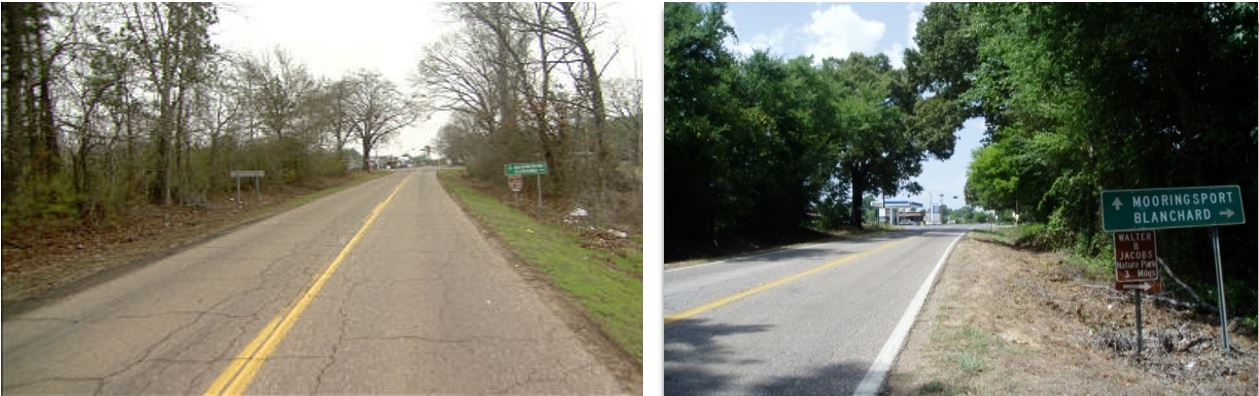
\includegraphics[width=10.5in, height= 3in]{abc.jpg}
                %\caption{Crash reductions by weather conditions.}
                %\label{fig:multDom}
              \end{center}
      \end{figure}
      \begin{block}{Abstract}
        {\rmfamily{This research aims to investigate the application of zero-inflated models for different severity types in rural two-lane highway crashes in Louisiana. These roadways carry one-third of the total vehicle miles traveled (VMT) and have experienced a considerably high percentage of fatal crashes in Louisiana. Crashes recorded from 2004 to 2011, of which 1,780 were fatal, and 36,569 resulted in injuries, were analyzed. It is found that there are a large number of highway segments which contain no crashes under the recorded years. To tackle this issue, zero-inflated models, zero-inflated Poisson (ZIP) models and zero-inflated negative binomial (ZINB) models, have been developed for crash frequencies of different severity types.}}
      \end{block}
      \vskip2ex

      \begin{block}{Background}
        {\rmfamily{The State of Louisiana controls 60,937 miles of public road serving nearly 105,000 vehicle miles a day, and consisting of 46,959 miles of rural roads and 13,941 miles of urban roads. Nearly 58,000 miles of undivided rural roadways are two-lane in nature. Each year, approximately 150,000 crashes occur, over 90,000 of which are on the state-maintained highway system. In 2013, 703 people were killed and 70,658 were injured in highway crashes in Louisiana. Zero-inflated models, zero-inflated Poisson (ZIP) and zero-inflated negative binomial (ZINB), have been developed in this study for crash frequencies of different severity types. }}
      \end{block}
    \end{column}

   \begin{column}{\sepwid}\end{column}			% empty spacer column
    \begin{column}{\twocolwid}							% create a two-column-wide column and then we will split it up later
      \begin{columns}[t,totalwidth=\twocolwid]	% split up that two-column-wide column

        \begin{column}{\onecolwid}\vspace{-.69in}
          \begin{block}{Data Description}
             {\rmfamily{Eight years (2004-2011) of Louisiana crash data was used in this study. }}
             \begin{itemize}
              \item The important roadway factors considered in the study include segment length, pavement type and width, shoulder type and width, and annual average daily traffic (AADT).
              \item There are a total of 7,779 rural two-lane roadway segments in each year\textquotesingle s crash dataset. The key variables available in the current dataset, related to roadway geometrics, were considered here. Louisiana Department of Transportation and Development (LaDOTD) has been maintaining crash data which doesn\textquotesingle t have details on other roadway geometrics like vertical and horizontal curve degree, deflection angle, and percentage of gradient.
            \end{itemize}
            \vspace{0.25in}
            \begin{figure}
              \begin{center}
                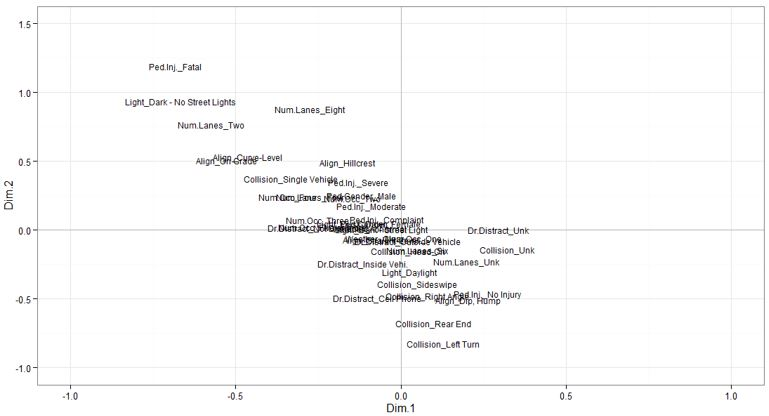
\includegraphics[width=10in]{m2.jpg}
                \caption{Crash frequencies of different severity types.}
                \label{fig:multDom}
              \end{center}
            \end{figure}
          \end{block}
        \end{column}
        \begin{column}{\onecolwid}\vspace{-.69in}
                  \begin{block}{Zero Inflated Models}
            {\rmfamily{Crash-frequency data are non-negative integers, the application of the standard ordinary least-squares regression (which assumes a continuous dependent variable) is not appropriate. }}\\
            \vspace{0.25in}

        {\rmfamily{
             The ZIP and ZINB regressions directly model the zeroes in the structural portion of the model. These models are generally considered as mixture models in which the complete distribution of the outcome is approximated by mixing two component distributions. The basic idea is to assume a logistic regression model for the \textbf{zero, and not zero} aspect of the consequence and either a Poisson or negative binomial distribution for the count portion in the model. ZIP and ZINB are well suited for the models in which there are two procedures and where the factors of the two procedures vary.}}

            \begin{figure}
              \begin{center}
                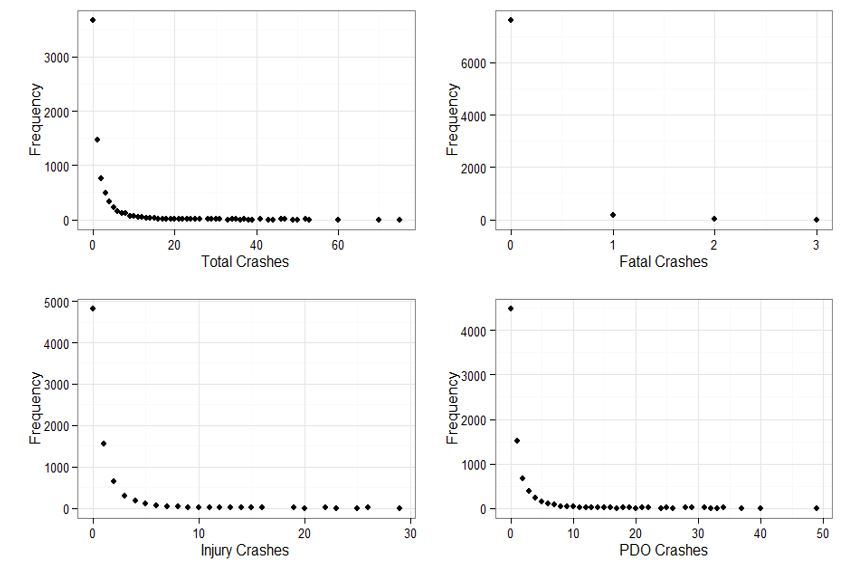
\includegraphics[width=10in]{m1.jpg}
                \caption{Crash frequency of different count of crashes per segment.}
                \label{fig:multDom}
              \end{center}
            \end{figure}
          \end{block}
        \end{column}

\end{columns}
      \vskip4ex
      \begin{alertblock}{\textbf{Major Findings}}		% an ACTUAL two-column-wide column
          \begin{itemize}
          {\item Wider shoulder and pavement were found to reduce the likelihood of crash occurrence in rural two-lane highways.
              \item Gravel-top pavements are inclined to crash proneness according to both of the models.
              \item Lower values of AADT is significant for reducing the likelihood of crashes.
              \item When the test statistic value > 1.96 (the 95\% confidence level for the t-test), the ZINB or ZIP model is more significant than traditional negative binomial or Poisson model.
}
            \end{itemize}
      \end{alertblock}
\end{column}

  \begin{column}{\sepwid}\end{column}			% empty spacer column
  \begin{column}{\onecolwid}
    \begin{block}{Model Comparison}
            \begin{figure}
              \begin{center}
                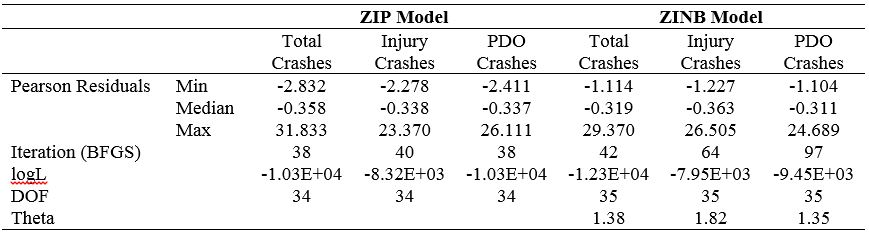
\includegraphics[width=10.5in, height= 3.5 in]{m3.jpg}

              \end{center}
            \end{figure}
    \end{block}
    \vskip2ex


        \begin{block}{Model Validation}
            \begin{figure}
              \begin{center}
                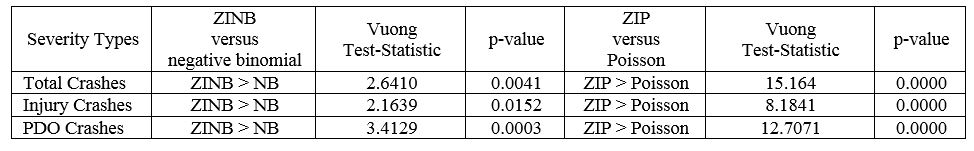
\includegraphics[width=10.5in, height=2.5in]{m4.jpg}
                %\caption{Significant Characteristics}
                %\label{fig:multDom}
              \end{center}
            \end{figure}
        \end{block}
    \vskip2ex



    \begin{block}{Limitations}
          \begin{itemize}
              {\item Although zero-inflated models offer improved statistical fit to crash data in many cases, it is argued that the inherent assumption of a dual state process underlying the development of these models is inconsistent with crash data
              \item This research aims to utilize ZIP and ZINB models to investigate the significance of the recoded categorical values of the geometric factors for traffic crashes of different severities which has not been done extensively in crash data analysis before. }
            \end{itemize}
    \end{block}
    \vskip2ex
        \begin{block}{Conclusions}
              {\rmfamily{
              Based on the test statistic, ZIP and ZINB models provided a better fit than conventional Poisson or negative binomial model for total, injury and PDO crashes. One future scope of this research is to introduce non-parametric statistical methods to the extended dataset to compare the statistical significance.}}



      \begin{center}
        \begin{tabular}{ccc}
          
\includegraphics[width=3in, height=3in]{ulls.jpg}
        \end{tabular}
      \end{center}
    \end{block}
  \end{column}
  \begin{column}{\sepwid}\end{column}			% empty spacer column
 \end{columns}
\end{frame}
\end{document}
